\chapter{Введение в доверительное оценивание} 

Пусть наблюдение $ X = (X_1, \ldots, X_n), \; X \sim P_{\theta}, \; \theta \in \Theta \in \mathbb{R}^1, \; \Theta $ -- интервал. Пусть $ T_1(X) \leq T_2(X), \; (T_1(X), T_2(X)) \subseteq \Theta $.

\begin{definition}
	Если $ P_{\theta}(T_1(X) < \theta < T_2(X)) \geq 1 - \alpha \;\; \forall \theta \in \Theta $, то случайный интервал $ (T_1(X), T_2(X)) $ называется \red{доверительным интервалом уровня $ 1 - \alpha $}, $ 0 < \alpha < 1 $.
\end{definition}

Интервал $ (T_1(X), T_2(X)) $ можно понимать как интервальную оценку (в отличие от точечной) параметра $ \theta $. Он покрывает неизвестное $ \theta $ с вероятностью, не меньшей, чем $ 1 - \alpha$.

\section{Доверительные интервалы для параметров Гауссовских выборок}

\subsection*{Доверительный интервал для среднего $ a $ при известной дисперсии $ \sigma^2 $}

$ X = (X_1, \ldots, X_n), \; \lbrace X_i \rbrace $ -- н.о.р., $ X_1 \sim N(a, \sigma^2) $.

Оптимальная оценка для $ a $ -- $ \bar{X} \sim N(a, \dfrac{\sigma^2}{n}) $. Значит, $ \dfrac{n^{\frac{1}{2}}(\bar{X} - a)}{\sigma} \sim N(0, 1) $. Пусть $ \phi(x) $ -- функция распределения $ N(0, 1) $, то есть $ \phi(x) = \dfrac{1}{\sqrt{2 \pi}} \int\limits_{- \inf}^x e^{-\frac{t^2}{2}}dt $. Пусть $ \xi_{\alpha}: \phi(\xi_{\alpha}) = \alpha, \; 0 < \alpha < 1 $.

Тогда $ \forall a \; P_a(|\dfrac{n^{\frac{1}{2}}(\bar{X} - a)}{\sigma}| < \xi_{1 - \frac{\alpha}{2}}) = 1 - \alpha, $ то есть с вероятностью $ 1 - \alpha$:
$$ -\xi_{1 - \frac{\alpha}{2}}< \dfrac{n^{\frac{1}{2}}(\bar{X} - a)}{\sigma} < \xi_{1 - \frac{\alpha}{2}}, \; \bar{X} - \dfrac{\sigma\xi_{1 - \frac{\alpha}{2}}}{\sqrt{n}} < a <  \bar{X} + \dfrac{\sigma\xi_{1 - \frac{\alpha}{2}}}{\sqrt{n}}$$

\begin{center}
	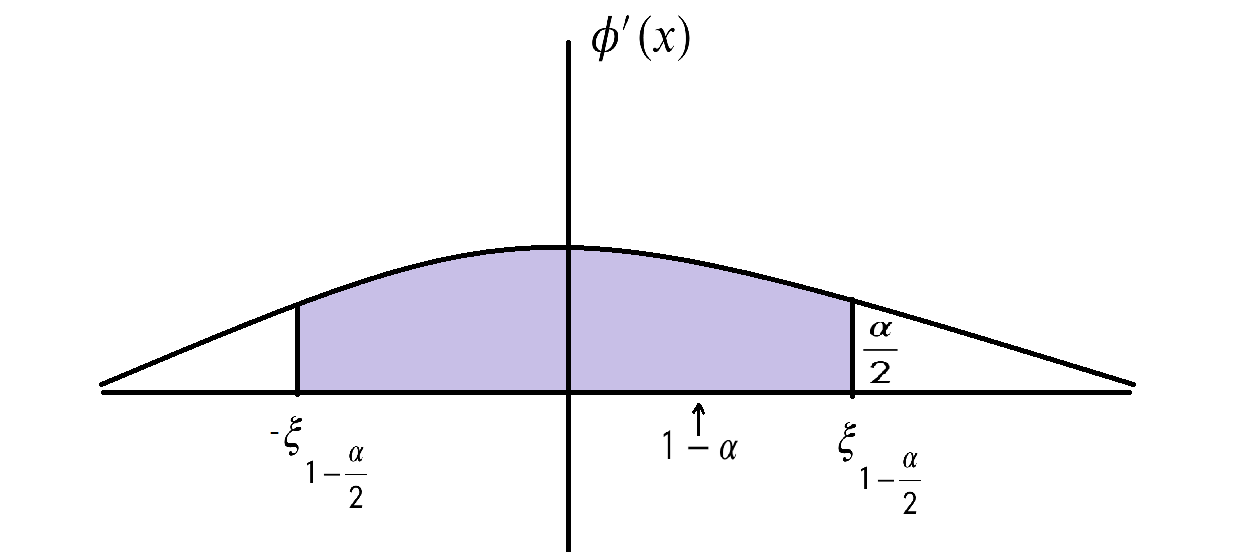
\includegraphics[scale=0.4]{N}

	$ \xi_{1 - \frac{\alpha}{2}} = -\xi_{\frac{\alpha}{2}} $
\end{center}

Интервал: 
$$ (\bar{X} - \dfrac{\sigma\xi_{1 - \frac{\alpha}{2}}}{\sqrt{n}}, \bar{X} + \dfrac{\sigma\xi_{1 - \frac{\alpha}{2}}}{\sqrt{n}}) \eqno(1)$$ 
называется \red{доверительным интервалом уровня $ 1 - \alpha $}, его длина $ ln = \dfrac{2\sigma\xi_{1 - \frac{\alpha}{2}}}{\sqrt{n}} $ю

\begin{property}
	Имеем несколько свойств:
	\begin{itemize}
		\item[$1)$] 
			$ \alpha \to 0 \; \Rightarrow \;  \xi_{1 - \frac{\alpha}{2}} \to \inf \; \Rightarrow \;  ln \to \inf $.
			\begin{remark}
				Обычно $ \alpha = 0.05, \; 0.01, \ldots $ и $ \alpha $ фиксировано.
			\end{remark}
		\item[$2)$] 
			$ n \to \inf \; \Rightarrow \;  ln \to 0 $.
		\item[$3)$] 
			$ \sigma \to 0 \; \Rightarrow \;  ln \to 0. $
	\end{itemize}
\end{property}

\begin{remark}
	Доверительных интервалов много. Например, $ \dfrac{X_1 - \theta}{\sigma} \sim N(0, 1) $, и на этой статистике можно построить доверительный интервал уровня $ 1 - \alpha $.
\end{remark}

\textit{Какой доверительный интервал наилучший?}

\begin{definition}
Доверительный интервал $ (T_1, T_2) $ уровня $ 1 - \alpha $ называется \red{несмещенным}, если $ P_{\theta}(T_1 < \theta' < T_2) \leq 1 - \alpha \; \forall \theta, \; \theta' $ таких, что $ \theta \neq \theta' $. То есть вероятность накрытия неверного параметра всегда \textbf{не больше} вероятности накрытия верного параметра.
\end{definition}

\begin{definition}
Несмещенный доверительный интервал $ (T_1, T_2) $ уровня $ 1 - \alpha $ называется \red{наиболее точным}, если он минимизирует вероятность $ P_{\theta}(T_1 < \theta' < T_2) \; \forall \theta, \; \theta' $ таких, что $ \theta \neq \theta' $ в классе всех \textbf{несмещенных} доверительных интервалов $ (T_1, T_2) $ уровня $ 1 - \alpha $.
\end{definition}

Можно показать, что (1) является наиболее точным несмещенным доверительным интервалом уровня $ 1 - \alpha $, то есть \textit{оптимальным}.

\subsection*{Доверительный интервал для среднего $ a $ при неизвестной дисперсии $ \sigma^2 $}
 
$ X = (X_1, \ldots, X_n), \; \lbrace X_i \rbrace $ -- н.о.р., $ X_1 \sim N(a, \sigma^2), \; n \geq 2 $.

\begin{definition}\label{cha:9/def:1}
	Если $ \xi_0, \ldots, \xi_k $ -- н.о.р. N(0, 1) сл.в., то сл.в. $$ \begin{gathered} t_k = \dfrac{\xi_0}{\sqrt{\dfrac{1}{k}(\xi_1^2 + \ldots + \xi_k^2)}} \end{gathered} $$ имеет \blue{распределение Стьюдента с к степенями свободы}. \textit{Обозначение:} $ t_k \sim S(k)$.
\end{definition}

Очевидно, $ t_k = \dfrac{\xi_0}{\sqrt{\frac{1}{k}\eta_k}}, \text{ где } \xi_0, \; \eta_k  $ независимы, $ \eta_k \sim \chi^2(k). $\\

Пусть $ S_k(x) := P(t_k \leq x) $ -- ф.р. $ t_k .$ Пусть $ S_k(t_{\alpha}(k)) = \alpha, \; 0 < \alpha < 1,  $ то есть $ t_{\alpha}(k) $ -- \red{квантиль уровня $ \alpha $ ф.р. $ S_k(x) $}. Поскольку $ t_k \stackrel{d}{t_k} $, то плотность вероятности $ S_k(x)' $ -- четная функция. Значит, $ -t_{\alpha}(x) = t_{1 - \alpha}(x) $.

Известно, что $ \bar{X} $ и $ s^2 $ -- оптимальные оценки $ a, \; \sigma^2 $, $ \bar{X} $ и $ s^2 $ независимы, 
$$ \begin{gathered} \dfrac{n^{\frac{1}{2}}(\bar{X} - a)}{\sigma} \sim N(0, 1), \; \dfrac{(n - 1)s^2}{\sigma^2} \sim \chi^2(n - 1) \end{gathered} $$ 
Здесь $ s^2 = \dfrac{1}{n -1}\sum\limits_{i = 1}^{n}(X_i - \bar{X}).  $ Значит: 
$$ \begin{gathered} \dfrac{n^{\frac{1}{2}}(\bar{X} - a)}{\sigma} / \sqrt{\dfrac{1}{n - 1} \dfrac{(n - 1)s^2}{\sigma^2}} = \dfrac{n^{\frac{1}{2}}(\bar{X} - a)}{s} \sim S(n - 1).  \end{gathered}$$
Значит: $$ \begin{gathered} P_{a, \sigma^2}(|\dfrac{n^{\frac{1}{2}}(\bar{X} - a)}{s}|) < t_{1 - \frac{\alpha}{2}}(n - 1) = 1 - \alpha. \end{gathered} $$ Получаем доверительный интервал уровня $ 1 - \alpha: $ $$ \begin{gathered} \bar{X} - \dfrac{st_{1 - \frac{\alpha}{2}}(n - 1)}{\sqrt{n}} < a < \bar{X} + \dfrac{st_{1 - \frac{\alpha}{2}}(n - 1)}{\sqrt{n}} \end{gathered} $$

\subsection*{Доверительный интервал для дисперсии $ \sigma^2 $ при неизвестном среднем $ a $}

$ X = (X_1, \ldots, X_n), \; \lbrace X_i \rbrace $ -- н.о.р., $ X_1 \sim N(a, \sigma^2), \; n \geq 2 $. 

Знаем, что $ \dfrac{(n - 1)s^2}{\sigma^2} \sim \chi^2(n - 1). $ Обозначим за $ \chi_{(n - 1)}(x) $ ф.р. $ \chi^2(n - 1), \; x_{\alpha}(n - 1) $ -- квантиль уровня $ \alpha, $ то есть $ \chi_{(n - 1)}(x_{\alpha}(n - 1)) = \alpha, \; 0 < \alpha < 1.$ Тогда $ P_{a, \sigma^2}(x_{\frac{\alpha}{2}}) < \dfrac{(n - 1)s^2}{\sigma^2} < x_{1 - \frac{\alpha}{2}}(n - 1)) = 1 - \alpha .$ Доверительный интервал уровня $ 1 - \alpha $: $$ \begin{gathered} \dfrac{(n - 1)s^2}{x_{1 - \frac{\alpha}{2}}(n - 1)} < \sigma^2 < \dfrac{(n - 1)s^2}{x_{\frac{\alpha}{2}}(n - 1)} \end{gathered} $$

\section{Оценивание параметров линейной регрессии}

Если $ \eta_k \sim \chi^2(k), \; \upsilon_m \sim \chi^2(m),  $ $ \eta_k $ и $ \upsilon_m $ независимы, то сл.в. $ f_{k, m} = \dfrac{\frac{1}{k}\eta_k}{\frac{1}{m}\upsilon_m} $ имеет распределение Фишера с $ (k, m) $ степенями свободы. Пишем $ f_{k, m} \sim F(k, m). $ Пусть $ F_{k, m}(x) $ -- ф.р., то есть $ F_{k, m}(f_{\alpha}(k, m)) = \alpha, \; 0 < \alpha < 1 $. 

\begin{lemma}\label{cha:9/lemma:1}
Если $ \xi \in \mathbb{R}^k, \; \xi \sim N(0, \Sigma), \; \Sigma > 0, $ то $ \sigma^T\Sigma^{-1}\sigma \sim \chi^2(k) $.
\end{lemma}
\begin{Proof}
	$$ \begin{gathered} \sigma^T\Sigma^{-1}\sigma = (\Sigma^{-\frac{1}{2}}\xi)^T(\Sigma^{-\frac{1}{2}}\xi) = |\Sigma^{-\frac{1}{2}}\xi|^2 \end{gathered} $$
	При этом $ \eta := \Sigma^{-\frac{1}{2}}\xi \sim N(0, E_k), $ так как $ \eta $ -- гаусс. Тогда: 
	$$ \begin{gathered} 
		E\eta = \Sigma^{-\frac{1}{2}}E\eta = 0, \; Cov(\eta, \eta) = E\eta\eta^T = \Sigma^{-\frac{1}{2}}\Sigma\Sigma^{-\frac{1}{2}} = E_k, \\
		\text{т.е. } |\Sigma^{-\frac{1}{2}}\xi|^2 = |\eta|^2 = \eta_1^1 + \ldots + \eta_k^2 \sim \chi^2(k)
	\end{gathered} $$
\end{Proof}

Рассмотрим регрессию $ X = Zc + \varepsilon, \; \varepsilon \sim N(0, \sigma^2E_n) $. Пусть $ \hat{c_n} $ -- о.н.к. для $ c, \; \hat{s_n}^2 $ -- о.н.к. для $ \sigma^2 $.

Тогда известно, $ \hat{c_n} \sim N(c, \sigma^2(Z^TZ)^{-1}), \dfrac{(n - p)\hat{s_n}}{\sigma^2} \sim \chi^2(n - p), $ $ \hat{c_n} $ и $ \hat{s_n}^2 $ независимы. Значит, в силу леммы \ref{cha:9/lemma:1}: 
$$ \begin{gathered} 
	\dfrac{1}{\sigma^2}(\hat{c_n} - c)^T(Z^TZ)(\hat{c_n} - c) \sim \chi^2(p), \\ f_{p, n - p} := \dfrac{\frac{1}{p}\frac{1}{\sigma^2}(\hat{c_n} - c)^T(Z^TZ)(\hat{c_n} - c)}{\frac{1}{n - p}\frac{(n - p)\hat{s_n}^2}{\sigma^2}} = \dfrac{(\hat{c_n} - c)^T(Z^TZ)(\hat{c_n} - c)}{p\hat{s_n}^2} \sim F(p, n - p)
\end{gathered} $$ 
Значит: 
$$ \begin{gathered} 
	P_{c, \sigma^2}((\hat{c_n} - c)^T(Z^TZ)(\hat{c_n} - c) \leq p\hat{s_n}^2f_{1 - \alpha}(p, n - p)) = 1 - \alpha 
\end{gathered} $$ 

\red{Доверительный эллипсоид уровня $ 1 - \alpha $}: 
$$ \begin{gathered} \lbrace c: \; (\hat{c_n} - c)^T(Z^TZ)(\hat{c_n} - c) < p\hat{s_n}^2f_{1 - \alpha}(p, n - p)\rbrace \end{gathered} $$ 
\textit{ Он накрывает неизвестный c с вероятностью $ 1 - \alpha $}.\\

Пусть $ c = (c_1, \ldots, c_p)^T, \; \hat{c_n} = (\hat{c_1}, \ldots, \hat{c_p})^T,  $ тогда $ \hat{c_{in}} \sim N(c_i, \sigma^2a_{ii}),  $ где $ (Z^TZ)^{-1} = (a_{ij}), \; i,j = 1, \ldots, p. $ Так как $ \hat{c_{in}} $ и $ \hat{s_n}^2$ независимы, то $$ t_{n - p}:= \dfrac{\hat{c_{in}} - c_i}{\sqrt{\sigma^2a_{ii}}} / \sqrt{\dfrac{1}{n - p}\dfrac{(n - p)\hat{s_n}^2}{\sigma^2}} = \dfrac{\hat{c_{in}} - c_i}{\hat{s_n}\sqrt{a_{ii}}} \sim S(n - p). $$

Доверительный интервал для $ c_i $ уровня $ 1 - \alpha :$ $$ \begin{gathered} \hat{c_{in}} - \hat{s_n}\sqrt{a_{ii}}t_{1 - \frac{\alpha}{2}}(n - p) < c_i < \hat{c_{in}} + \hat{s_n}\sqrt{a_{ii}}t_{1 - \frac{\alpha}{2}}(n - p) \end{gathered} $$.

\section{Ассимптотический доверительный интервал}

Пусть для неизвестного параметра $ \theta \in \Theta \in \mathbb{R}^1  $ существует ассимптотически нормальная оценка $ \hat{\theta_n} $, то есть:
$$n^{\frac{1}{2}}(\hat{\theta_n} - \theta) \stackrel{d}{\longrightarrow} N(0, \sigma^2(\theta)), \; n \to \inf \eqno(2)$$.

Предположим, что $ \sigma^2(\theta) > 0 \; \forall \theta \in \Theta$ и $ \sigma^2(\theta) $ непрерывна по $ \theta $. В силу (2) $ \hat{\theta_n} - \theta = n^{-\frac{1}{2}}n^{\frac{1}{2}}(\hat{\theta_n} - \theta) \stackrel{P}{\to} 0, \; n \to \inf, $ то есть $ \hat{\theta_n} $ -- состоятельная оценка $ \theta $. Значит: 
$$ \hat{\sigma_n}^2 := \sigma^2(\theta), \; n \to \inf \eqno(3)$$
В силу (2), (3) $ \dfrac{n^{\frac{1}{2}}(\hat{\theta_n} - \theta)}{\hat{\sigma_n}} \stackrel{d}{\to} N(0, 1), \; n \to \inf $. Значит, $ \displaystyle P_{\theta}(|\dfrac{n^{\frac{1}{2}}(\hat{\theta_n} - \theta)}{\hat{\theta_n}}| < \xi_{1 - \frac{\alpha}{2}}) \to 1 - \alpha, \; n \to \inf $.

Ассимптотический доверительный интервал уровня $ 1 - \alpha $ имеет вид: 
$$ \hat{\theta_n} - \dfrac{\hat{\sigma_n}\xi_{1 - \frac{\alpha}{2}}}{\sqrt{n}} < \theta <  \hat{\theta_n} + \dfrac{\hat{\sigma_n}\xi_{1 - \frac{\alpha}{2}}}{\sqrt{n}} $$ 
Он накрывает неизвестный параметр $ \theta $ прмерно с вероятностью $ 1 - \alpha $ при больших $ n $.

\section{Примеры}

\begin{example}
$ X = (X_1, \ldots, X_n), \; \lbrace X_i \rbrace $ -- н.о.р., $ X_1 \sim Pois(\theta), \; \theta > 0 $. Тогда $\displaystyle  n^{\frac{1}{2}}(\bar{X} - \theta) \stackrel{d}{\longrightarrow} N(0, \theta),  $ а т.к. $ \bar{X} \stackrel{P}{\longrightarrow} \theta,$ то $ \dfrac{n^{\frac{1}{2}}(\bar{X} - \theta)}{\sqrt{\bar{X}}} \stackrel{d}{\longrightarrow} N(0, 1) $. Ассимптотический доверительный интервал уровня $ 1- \alpha $: 
$$ \bar{X} - \dfrac{\sqrt{\bar{X}}\xi_{1 - \frac{\alpha}{2}}}{\sqrt{n}} < \theta <  \bar{X} + \dfrac{\sqrt{\bar{X}}\xi_{1 - \frac{\alpha}{2}}}{\sqrt{n}}$$
\end{example}

\begin{example}
$ X_1 \sim R(0, \theta), \; \theta > 0 $. 
$$ E_{\theta}X_1 = \dfrac{\theta}{2}, \; D_{\theta}X_1 = \dfrac{\theta^2}{12}, \; 2\bar{X} \stackrel{P}{\to} \theta, \; \dfrac{n^{\frac{1}{2}}(\bar{X}-\frac{\theta}{2})}{\frac{\theta}{2}\sqrt{3}} \stackrel{d}{\to} N(0, 1), \; n \to \inf$$ 
Значит: 
$$ \dfrac{\sqrt{3n}(2\bar{X} - \theta)}{\theta} \stackrel{d}{\to} N(0, 1), \; \dfrac{\sqrt{3n}(2\bar{X} - \theta)}{2\bar{X}} \stackrel{d}{\to} N(0, 1)$$

Ассимптотический доверительный интервал:
$$ 2\bar{X} - \dfrac{2\bar{X}\xi_{1 - \frac{\alpha}{2}}}{\sqrt{3n}} < \theta <  2\bar{X} + \dfrac{2\bar{X}\xi_{1 - \frac{\alpha}{2}}}{\sqrt{3n}}$$
\end{example}



































